\begin{prob}
    Suppose we are given a directed and weighted graph $G = (V, E)$ that look like the following figure. It is known that there are no negative cycles.

    \begin{center}
        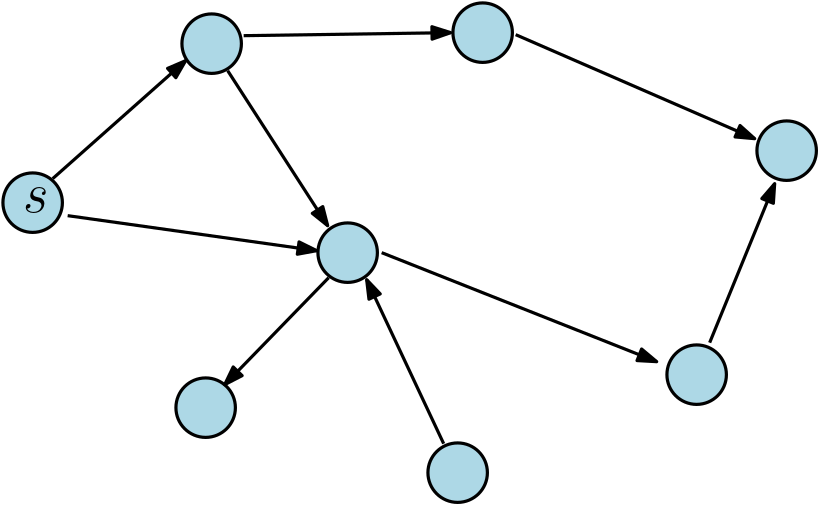
\includegraphics[scale=.4]{\thisdir/include/graphshape.png}
    \end{center}

    Suppose the Bellman-Ford algorithm {\bf with early stopping} is run on this graph shown above using node $s$ as the source (the edge weights are purposely not shown). In the worst case, how many iterations of the outer for-loop of Bellman-Ford will be performed?  Briefly justify your answer.

   \begin{soln}
        % write your solution here
   \end{soln}
\end{prob}
